\documentclass[11pt,compress,t,notes=noshow]{beamer}\usepackage[]{graphicx}\usepackage[]{color}

\makeatletter
\def\maxwidth{ %
  \ifdim\Gin@nat@width>\linewidth
    \linewidth
  \else
    \Gin@nat@width
  \fi
}
\makeatother

\definecolor{fgcolor}{rgb}{0.345, 0.345, 0.345}
\newcommand{\hlnum}[1]{\textcolor[rgb]{0.686,0.059,0.569}{#1}}%
\newcommand{\hlstr}[1]{\textcolor[rgb]{0.192,0.494,0.8}{#1}}%
\newcommand{\hlcom}[1]{\textcolor[rgb]{0.678,0.584,0.686}{\textit{#1}}}%
\newcommand{\hlopt}[1]{\textcolor[rgb]{0,0,0}{#1}}%
\newcommand{\hlstd}[1]{\textcolor[rgb]{0.345,0.345,0.345}{#1}}%
\newcommand{\hlkwa}[1]{\textcolor[rgb]{0.161,0.373,0.58}{\textbf{#1}}}%
\newcommand{\hlkwb}[1]{\textcolor[rgb]{0.69,0.353,0.396}{#1}}%
\newcommand{\hlkwc}[1]{\textcolor[rgb]{0.333,0.667,0.333}{#1}}%
\newcommand{\hlkwd}[1]{\textcolor[rgb]{0.737,0.353,0.396}{\textbf{#1}}}%
\let\hlipl\hlkwb

\usepackage{framed}
\makeatletter
\newenvironment{kframe}{%
 \def\at@end@of@kframe{}%
 \ifinner\ifhmode%
  \def\at@end@of@kframe{\end{minipage}}%
  \begin{minipage}{\columnwidth}%
 \fi\fi%
 \def\FrameCommand##1{\hskip\@totalleftmargin \hskip-\fboxsep
 \colorbox{shadecolor}{##1}\hskip-\fboxsep
     \hskip-\linewidth \hskip-\@totalleftmargin \hskip\columnwidth}%
 \MakeFramed {\advance\hsize-\width
   \@totalleftmargin\z@ \linewidth\hsize
   \@setminipage}}%
 {\par\unskip\endMakeFramed%
 \at@end@of@kframe}
\makeatother

\definecolor{shadecolor}{rgb}{.97, .97, .97}
\definecolor{messagecolor}{rgb}{0, 0, 0}
\definecolor{warningcolor}{rgb}{1, 0, 1}
\definecolor{errorcolor}{rgb}{1, 0, 0}
\definecolor{code}{rgb}{0.97, 0.96, 1.0}
\newenvironment{knitrout}{}{} % an empty environment to be redefined in TeX

\usepackage{alltt}
\usepackage[utf8]{inputenc}
\usepackage[ngerman]{babel}
\usepackage{dsfont}
\usepackage{verbatim}
\usepackage{amsmath}
\usepackage{amsfonts}
\usepackage{mathtools}
\usepackage{csquotes}
\usepackage{cmbright}
\usepackage{multirow}
\usepackage{longtable}
\usepackage{enumerate}
\usepackage[absolute,overlay]{textpos}
\usepackage{psfrag}
\usepackage{algorithm}
\usepackage{algpseudocode}
\usepackage{eqnarray}
\usepackage{bytefield}
\usepackage{animate}
\usepackage{tikz}
\usetikzlibrary{shapes,matrix,positioning,chains,arrows,shadows,decorations.pathmorphing,fit,backgrounds}
\usepackage{adjustbox}
\usepackage{colortbl}
\usepackage{tabularx} % for tables (incl. \hline)
\usepackage{arydshln} % Load after array, longtable, colortab and/or colortbl , otherwise problems with \hline in tabular env
\usepackage{etex} %increase registers for \dimenS to more than 256, otherwise we get "No room for a new \dimen"
\usepackage{graphicx}
\usepackage{booktabs} %used in epr lectures
\usepackage{bm} % bold greek letters
\usepackage{hyperref} % url citing
\usepackage{blkarray} % block arrays
\usepackage{listings} % block of code
\usepackage{xcolor} %colored math symbols
\usepackage{pgffor}
\usepackage{verbatimbox}
\usepackage{xcolor}

%some colors
\definecolor{checkgreen}{HTML}{18A126}
\definecolor{errorred}{HTML}{FF0000}
\definecolor{blockbg}{HTML}{F7F7F7}
\definecolor{gray}{HTML}{A0A0A0}

% basic latex stuff
\newcommand{\col}{\par\colorbox{code}{\parbox{\textwidth}{\theverbbox}}\par}
\newcommand{\eg}{e.\,g.\xspace} %for example
\newcommand{\ie}{i.\,e.\xspace} %that is to say...
\newcommand{\pkg}[1]{{\fontseries{b}\selectfont #1}} %fontstyle for R packages
\newcommand{\lz}{\vspace{0.5cm}} %vertical space
\newcommand{\oneliner}[1] % Oneliner for important statements
{\begin{block}{}\begin{center}\begin{Large}#1\end{Large}\end{center}\end{block}}
\def\SpAr{\quad \Rightarrow \quad}

%new environments
\newenvironment{vbframe}  %frame with breaks and verbatim
{
 \begin{frame}[containsverbatim,allowframebreaks]
}
{
\end{frame}
}

\newenvironment{vframe}  %frame with verbatim without breaks (to avoid numbering one slided frames)
{
 \begin{frame}[containsverbatim]
}
{
\end{frame}
}

\newenvironment{blocki}[1]   % itemize block
{
 \begin{block}{#1}\begin{itemize}
}
{
\end{itemize}\end{block}
}

\newenvironment{fragileframe}[2]{  %fragile frame with framebreaks
\begin{frame}[allowframebreaks, fragile, environment = fragileframe]
\frametitle{#1}
#2}
{\end{frame}}

\newcommand{\myframe}[2]{  %short for frame with framebreaks
\begin{frame}[allowframebreaks]
\frametitle{#1}
#2
\end{frame}}

\usepackage{../../style/lmu-lecture}

\let\code=\texttt
\let\proglang=\textsf

\setkeys{Gin}{width=0.9\textwidth}

\usepackage{tikz}
\usetikzlibrary{shapes,arrows,snakes, calc}

% Define block styles
\tikzstyle{decision} = [diamond, draw, text width=6em, text badly centered, node distance=4cm, inner sep=0pt]
\tikzstyle{decision2} = [diamond, draw, fill=customgreen!35, text width=6em, text badly centered, node distance=4cm, inner sep=0pt]

\tikzstyle{block} = [rectangle, draw, text width=14em, text centered, rounded corners, node distance=3cm, minimum height=4em]
\tikzstyle{line} = [draw, -latex']
\tikzstyle{cloud} = [draw, ellipse, node distance=3cm, minimum height=2em]

\title{Introduction to Deep Learning}
\author{Bernd Bischl}
\institute{Department of Statistics -- LMU Munich}
\date{WS 2021/2022}

\setbeamertemplate{frametitle}{\expandafter\uppercase\expandafter\insertframetitle}

\IfFileExists{upquote.sty}{\usepackage{upquote}}{}
\input{../../latex-math/basic-math}
\input{../../latex-math/basic-ml}
\input{../../latex-math/ml-nn}

\begin{document}
\lecturechapter{1}{Introduction}
\lecture{I2DL}
%%%%%%%%%%%%%%%%%%%%%%%%%%%%%%%%%%%%%%%%%%%%%%%%%%%%%%%%%%%%%%%%%%

\begin{frame} {What is Deep Learning}
\begin{center}
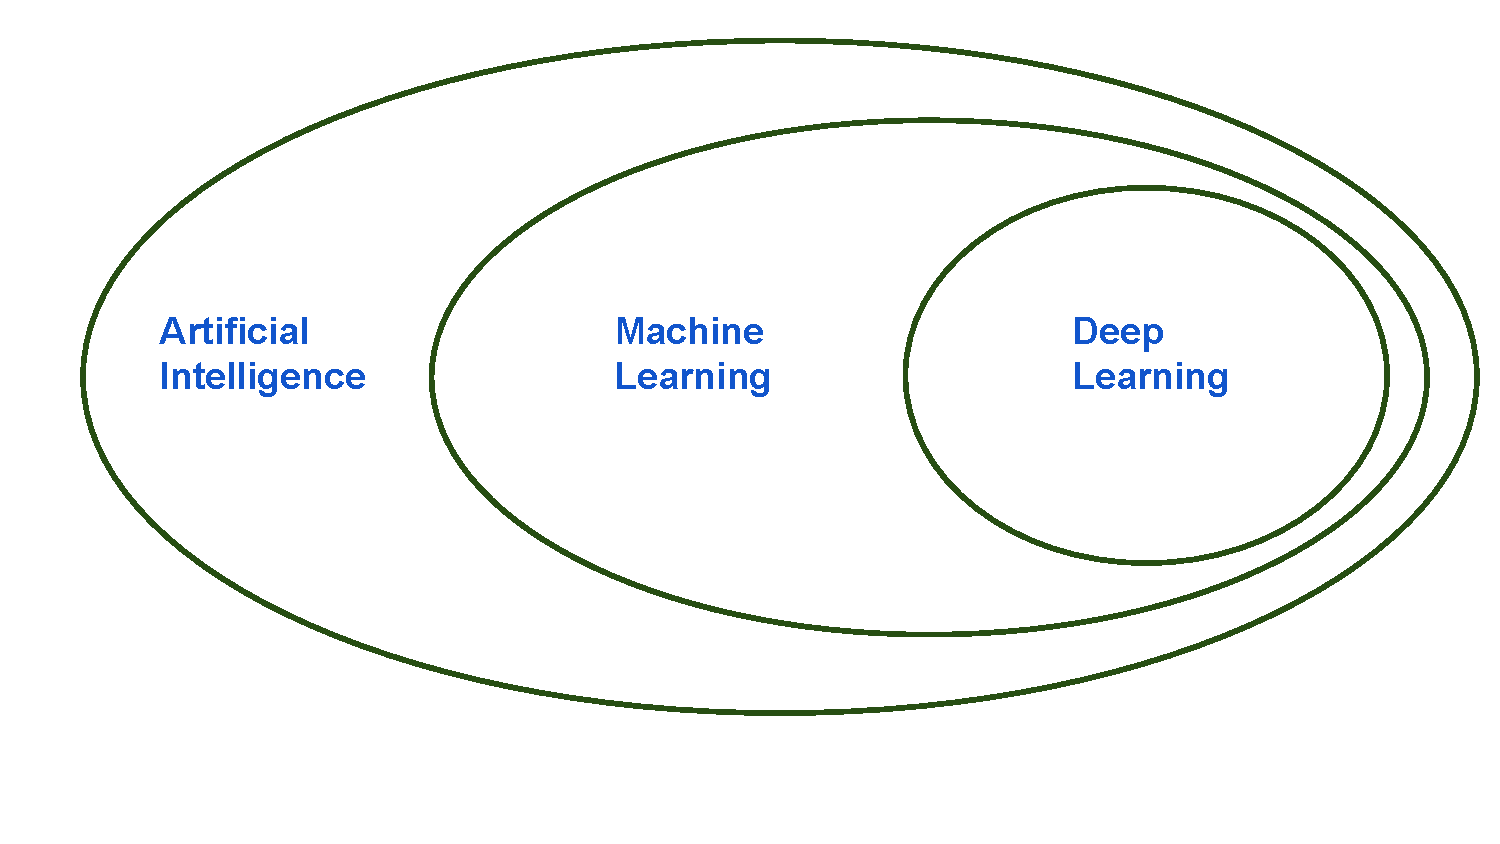
\includegraphics[width=0.95\textwidth]{figure/learning.pdf}
\end{center}
\vspace{-.5cm}
\begin{itemize}
\item Deep learning is the use of artificial neural networks to
construct models on large amounts of (unstructured) data.
\end{itemize}
\end{frame}
%%%%%%%%%%%%%%%%%%%%%%%%%%%%%%%%%%%%%%%%%%%%%%%%%%%%%%%%%%%%%%%%%%

\begin{frame} {Deep Learning and Neural Networks}
\begin{itemize}
\item Deep learning and neural networks are mostly equivalent.
\vspace{.3cm}
\item Deep learning itself is not \textit{new}:
\begin{itemize}
\item Neural networks have been around since the 70s
\item \textit{Deep} neural networks, i.e., networks with multiple hidden layers, are not much younger.
\end{itemize}
\vspace{.3cm}
\item Why everybody is talking about deep learning now:
\begin{enumerate}
\vspace{.1cm}
\item Specialized, powerful hardware allows training of huge neural networks to push the state-of-the-art on difficult problems.
\vspace{.2cm}
\item Large amount of data is available.
\vspace{.2cm}
\item Special network architectures for image/text data.
\vspace{.2cm}
\item Better optimization and regularization strategies.
\end{enumerate}
\end{itemize}
\end{frame}
%%%%%%%%%%%%%%%%%%%%%%%%%%%%%%%%%%%%%%%%%%%%%%%%%%%%%%%%%%%%%%%%%%

\begin{frame}{Image Classification with Neural Networks}
\begin{aquote}{Y. Bengio}
Machine learning algorithms, inspired by the brain, based on learning multiple levels of representation/abstraction.   
\end{aquote}
\begin{overlayarea}{\textwidth}{\textheight}
\centering
\only<1>{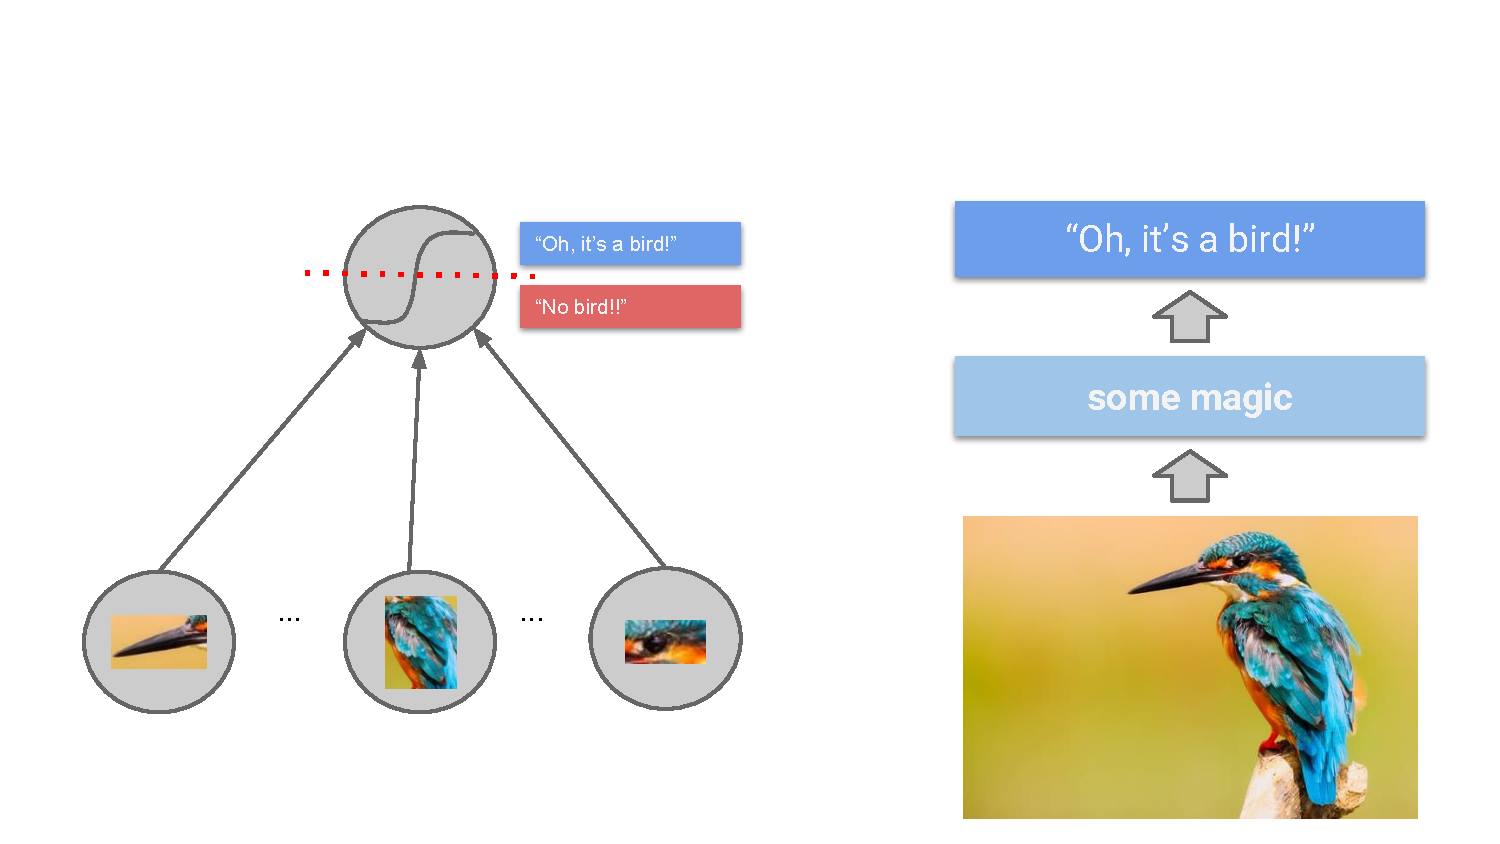
\includegraphics[width=0.7\textwidth]{figure/bird1.pdf}}
\only<1>{\\ \footnotesize{Caption 1}}
\only<2>{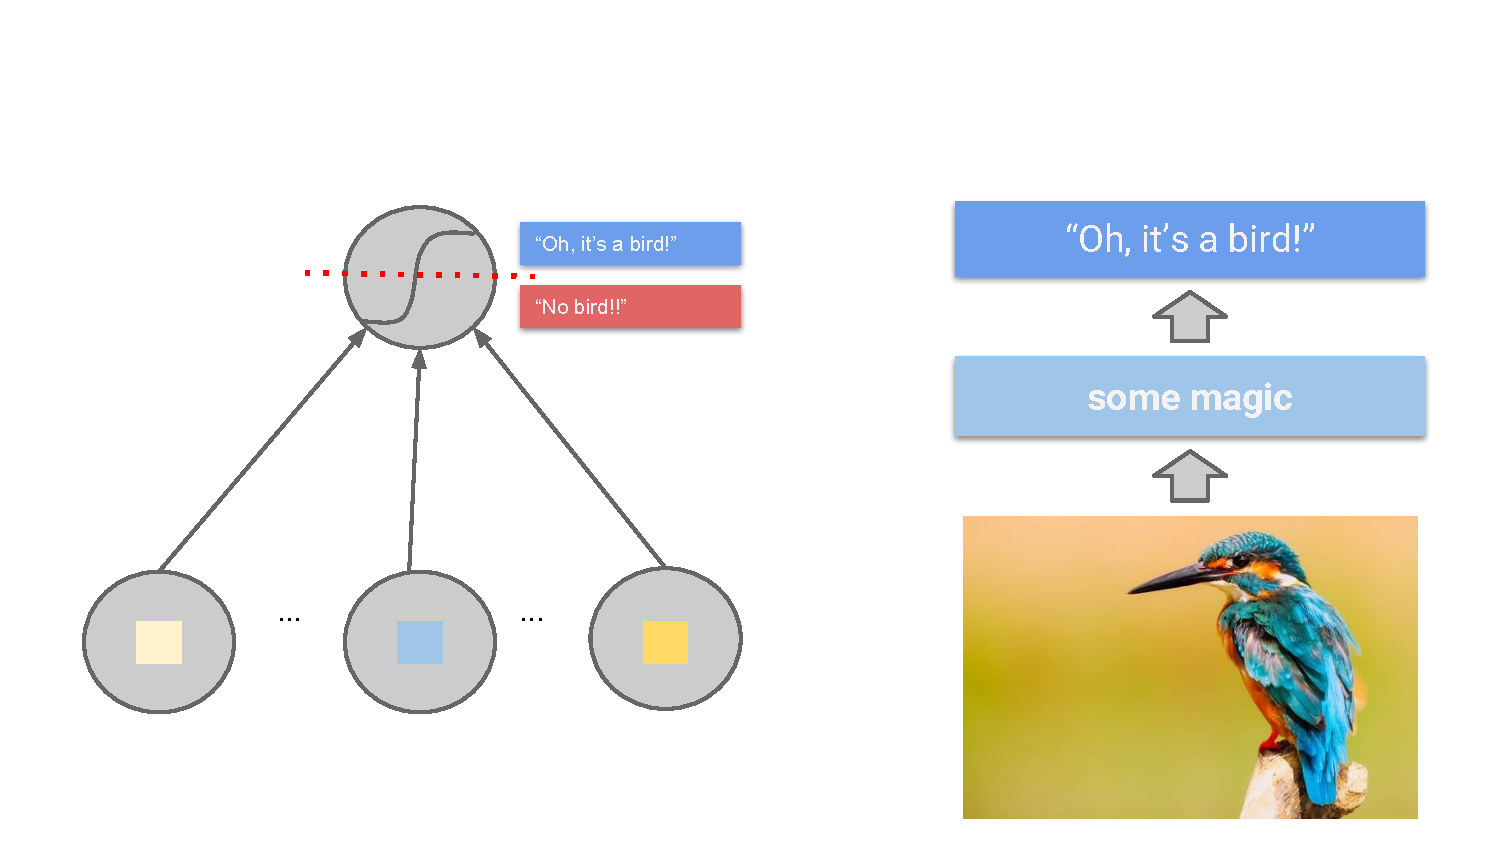
\includegraphics[width=0.7\textwidth]{figure/bird2.pdf}}
\only<2>{\\ \footnotesize{Caption 2}}
\only<3>{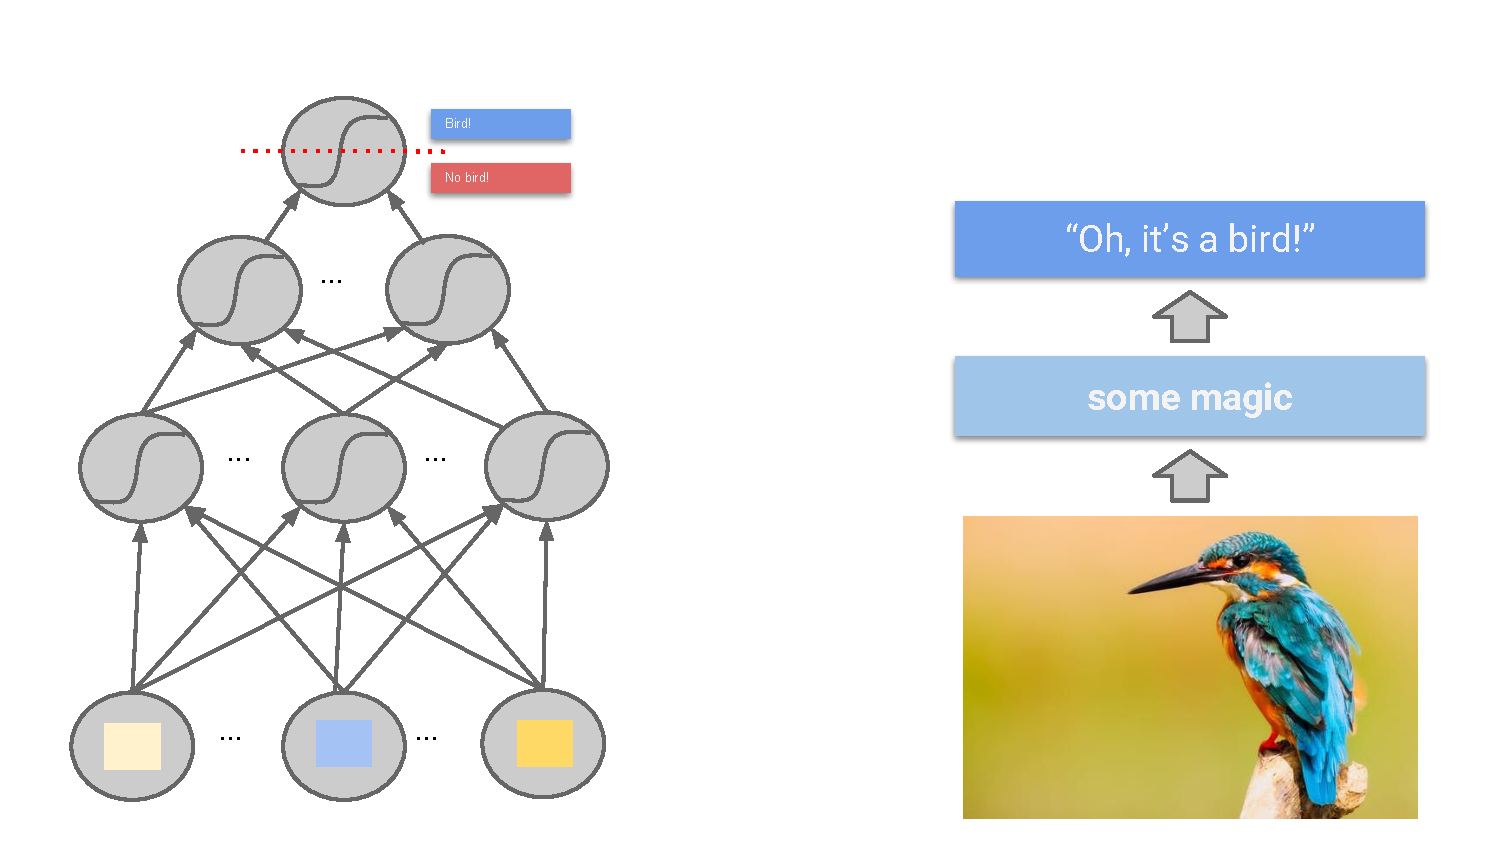
\includegraphics[width=0.7\textwidth]{figure/bird3.pdf}}
\only<3>{\\ \footnotesize{Caption 3}}
\only<4>{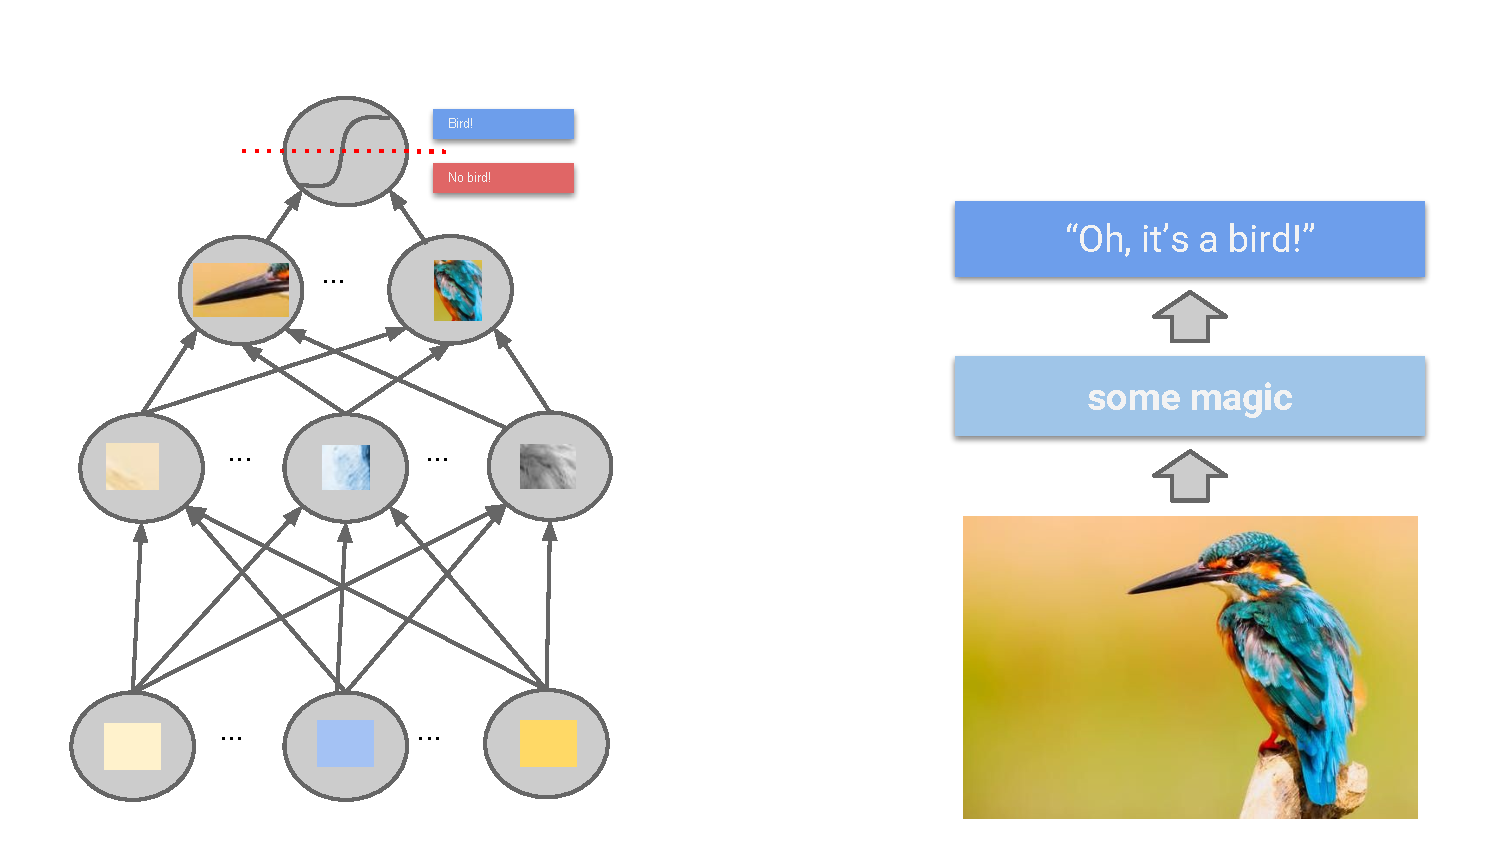
\includegraphics[width=0.7\textwidth]{figure/bird4.pdf}}
\only<4>{\\ \footnotesize{Caption 4}}
\end{overlayarea}
\end{frame}
%%%%%%%%%%%%%%%%%%%%%%%%%%%%%%%%%%%%%%%%%%%%%%%%%%%%%%%%%%%%%%%%%%

\begin{frame} {Possible use-cases}
\textbf{Deep learning can be extremely valuable if the data has these properties:}
\vspace{.2cm}
\begin{itemize}
\item It is high dimensional.
\item Each single feature itself is not very informative but only a combination of them might be.
\item There is a large amount of training data.
\end{itemize}
\vspace{.7cm}
\textbf{This implies that for tabular data, deep learning is almost never the correct model choice.}
\vspace{.2cm}
\begin{itemize}
\item Models like random forests or gradient boosting will outperform deep learning most of the time.
\item One exception is data with categorical features with many levels.
\end{itemize}

\end{frame}
%%%%%%%%%%%%%%%%%%%%%%%%%%%%%%%%%%%%%%%%%%%%%%%%%%%%%%%%%%%%%%%%%%

\begin{frame} {Possible use-case: Images}
\begin{itemize}
\item \textbf{High Dimensional}: A color image with $255 \times 255$ (3 Colors) pixels already has $195075$ features.
\vspace{.1cm}
\item \textbf{Informative}: A single pixel is not meaningful in itself.
\vspace{.1cm}
\item \textbf{Training Data}: Depending on applications huge amounts of data are available.
\end{itemize}
\vspace{.3cm}
Architecture: \textbf{C}onvolutional \textbf{N}eural \textbf{N}etworks (CNN)
\begin{figure}
\centering
\scalebox{.85}{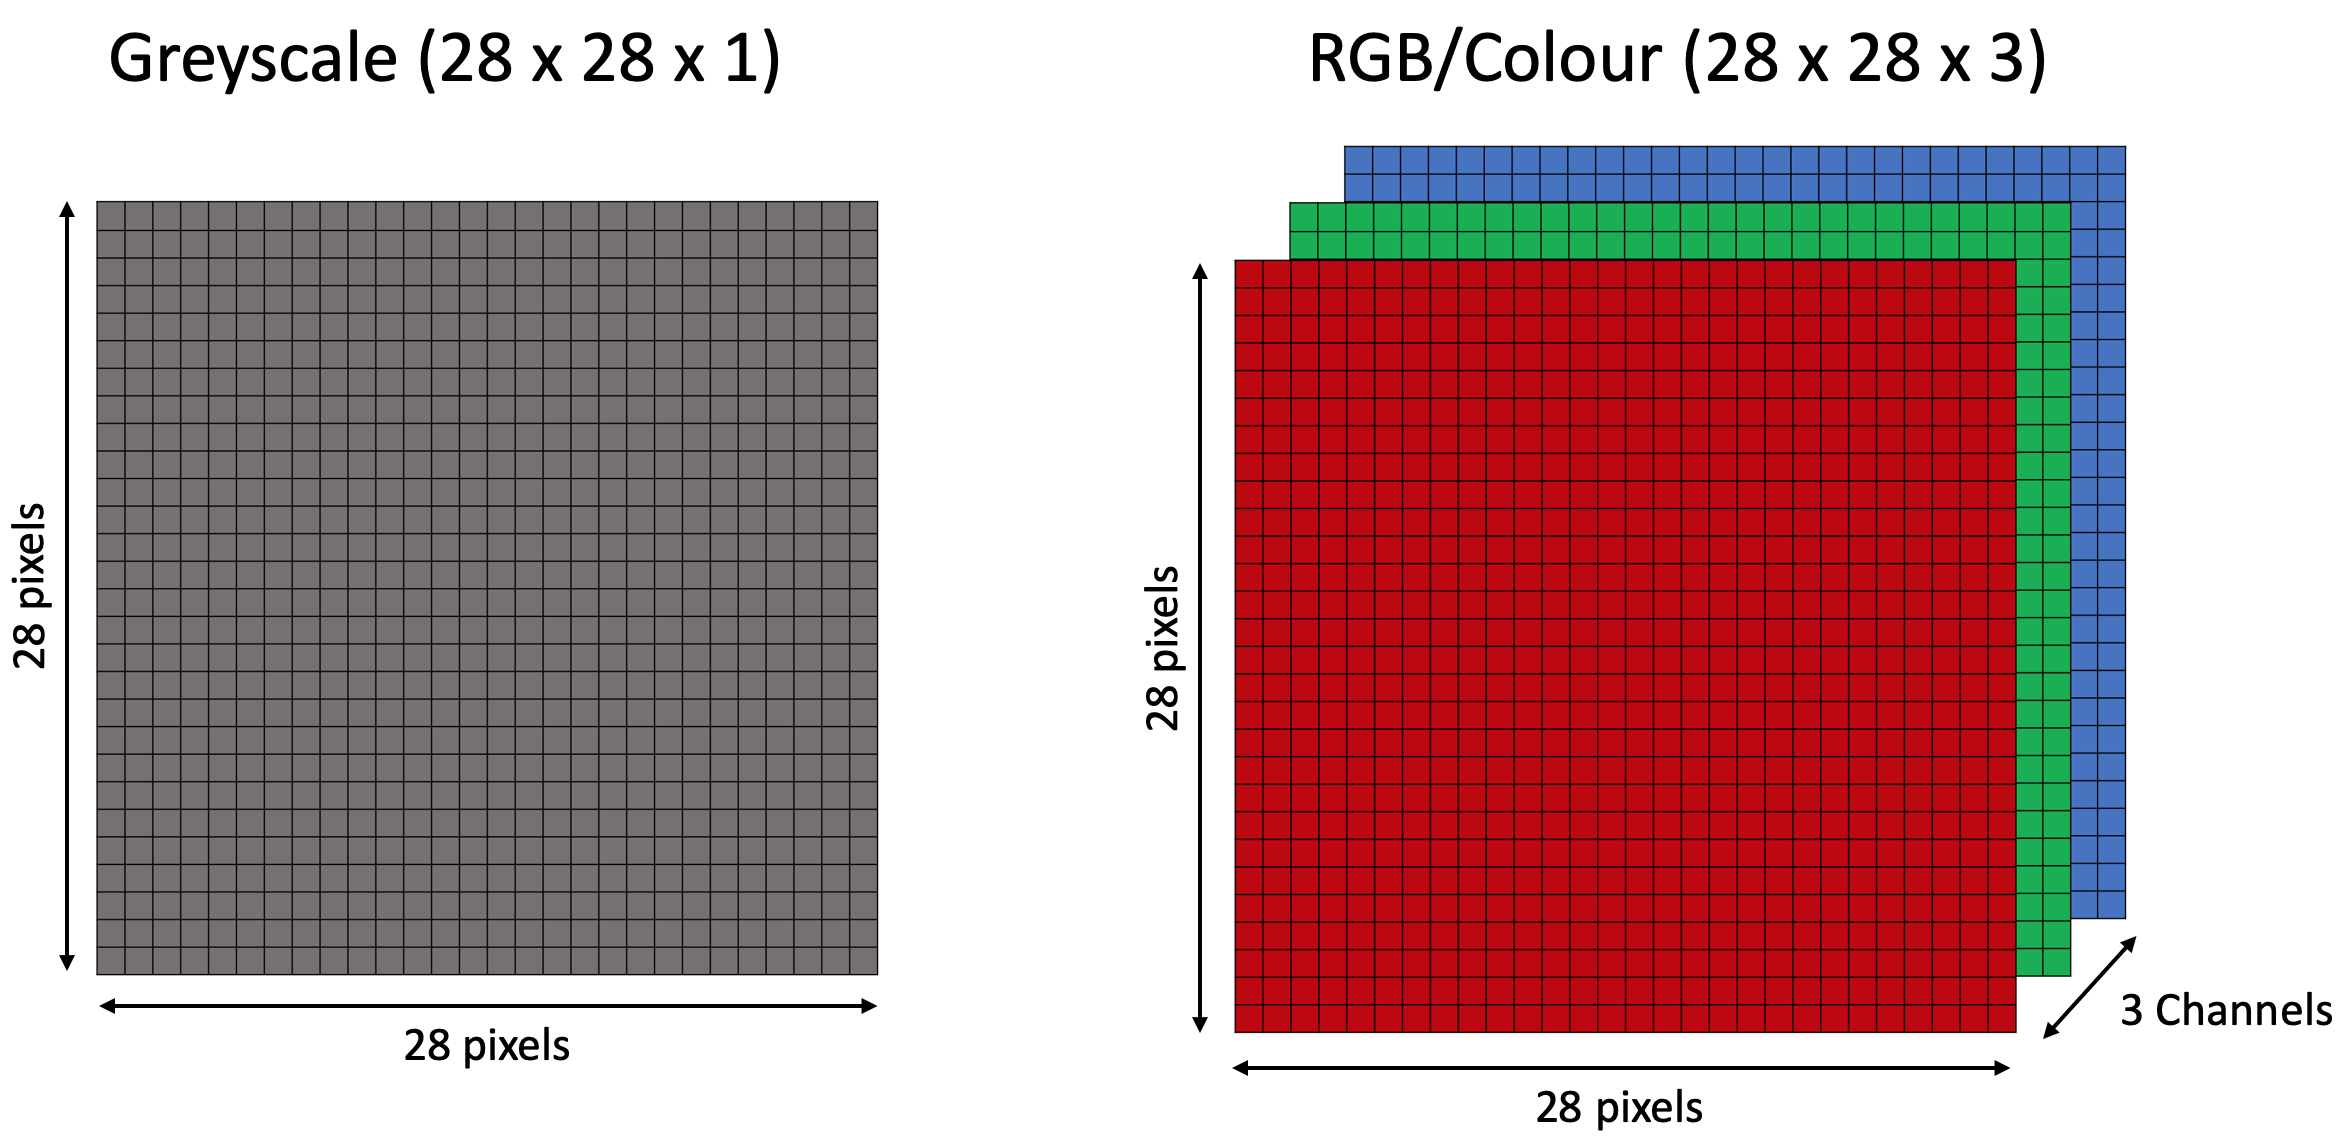
\includegraphics{figure/three_channels.png}}
\end{figure}
\end{frame}
%%%%%%%%%%%%%%%%%%%%%%%%%%%%%%%%%%%%%%%%%%%%%%%%%%%%%%%%%%%%%%%%%%

\begin{frame} {Possible use-case: Images}
\begin{figure}
\centering
\scalebox{.7}{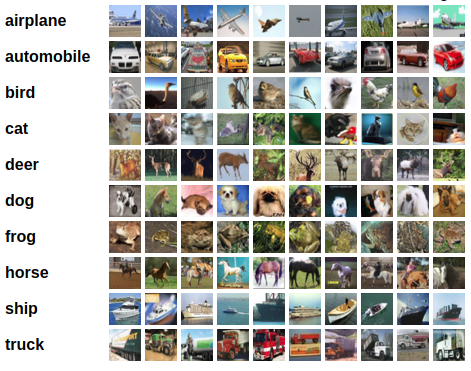
\includegraphics{figure/classification.png}}
\\
\tiny{Credit: Alex Krizhevsky (2009)}
\end{figure}
\textbf{Image classification} tries to predict a single label for each image.
\footnotesize CIFAR-10 is a well-known dataset used for image classification. It consists of $60,000$ $32x32$ color images containing one of $10$ object classes, with $6000$ images per class. 
\end{frame}
%%%%%%%%%%%%%%%%%%%%%%%%%%%%%%%%%%%%%%%%%%%%%%%%%%%%%%%%%%%%%%%%%%

\begin{frame} {Possible use-case: Images}
\begin{figure}
\centering
\scalebox{0.8}{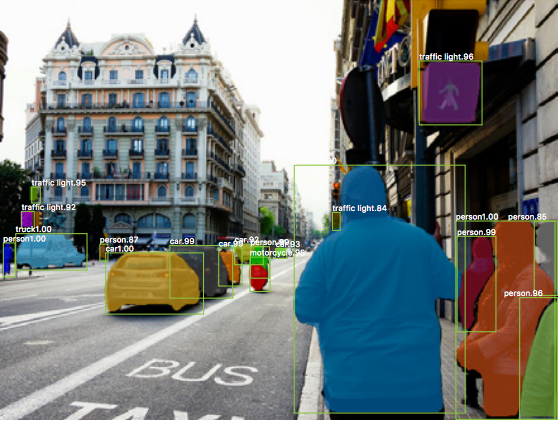
\includegraphics{figure/maskrcnn.png}}
\\
\tiny{Credit: Kaiming He (2017)}
\end{figure}
\textbf{Object Detection}
\footnotesize Mask R-CNN is a general framework for instance segmentation, which efficiently detects objects in an image while simultaneously generating a high-quality segmentation mask for each instance.
\end{frame}
%%%%%%%%%%%%%%%%%%%%%%%%%%%%%%%%%%%%%%%%%%%%%%%%%%%%%%%%%%%%%%%%%%

\begin{frame} {Possible use-case: Images}
\begin{figure}
\centering
\scalebox{.8}{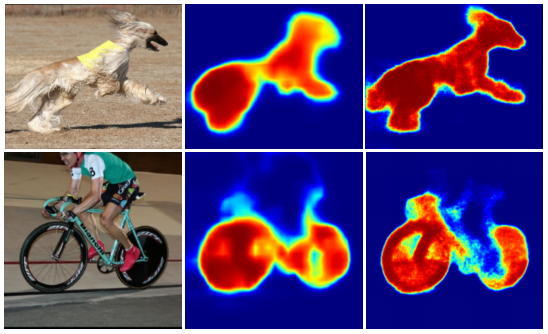
\includegraphics{figure/segmentation.png}}
\\
\tiny{Credit: Hyeonwoo Noh (2015)} 
\end{figure}
\textbf{Image segmentation} partitions the image into (multiple) segments.
\end{frame}
%%%%%%%%%%%%%%%%%%%%%%%%%%%%%%%%%%%%%%%%%%%%%%%%%%%%%%%%%%%%%%%%%%

\begin{frame} {Possible use-case: Text}
\begin{itemize}
\item \textbf{High Dimensional}: Each word can be a single feature (~300000 words in the German language).
\vspace{.1cm}
\item \textbf{Informative}: A single word does not provide much context.
\vspace{.1cm}
\item \textbf{Training Data}: Huge amounts of text data available.
\end{itemize}
\vspace{.3cm}
Architecture: \textbf{R}ecurrent \textbf{N}eural \textbf{N}etworks (RNN)
\begin{figure}
\centering
\scalebox{.75}{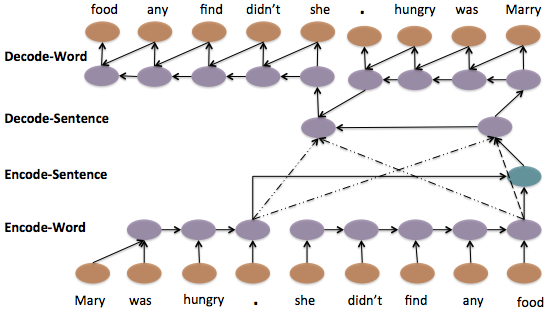
\includegraphics{figure/hierarchical_sequence.png}}
\end{figure}
\end{frame}
%%%%%%%%%%%%%%%%%%%%%%%%%%%%%%%%%%%%%%%%%%%%%%%%%%%%%%%%%%%%%%%%%%

\begin{frame} {Possible use-case: Text}
Applications:
\vspace{.7cm}
\begin{itemize}
\item \textbf{N}atural \textbf{L}anguage \textbf{P}rocessing, e.g.,
\begin{itemize}
\item Sentiment Analysis
\vspace{.3cm}
\item Email Classification
\vspace{.3cm}
\item Chat-bots
\vspace{.3cm}
\item $...$
\end{itemize}
\vspace{.7cm}
\item Modeling Sequential Data (Time-Series, Speech)
\end{itemize}
\end{frame}
%%%%%%%%%%%%%%%%%%%%%%%%%%%%%%%%%%%%%%%%%%%%%%%%%%%%%%%%%%%%%%%%%%

\begin{frame} {Possible use-case: Text}
\begin{figure}
\centering
\scalebox{.9}{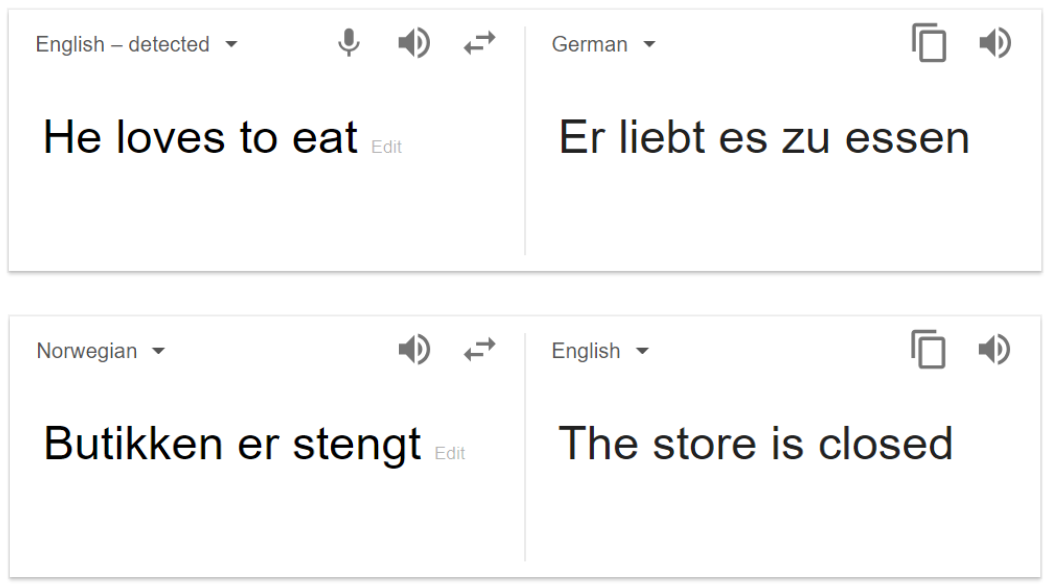
\includegraphics{figure/nmt.png}}
\end{figure}
\textbf{Machine Translation} (e.g. google translate) 
Neural machine translation exploits neural networks to predict the likelihood of a sequence of words, typically modeling entire sentences in a single integrated model.
\end{frame}
%%%%%%%%%%%%%%%%%%%%%%%%%%%%%%%%%%%%%%%%%%%%%%%%%%%%%%%%%%%%%%%%%%

\begin{frame} {Applications of Deep Learning: Speech}
\begin{figure}
\centering
\scalebox{.9}{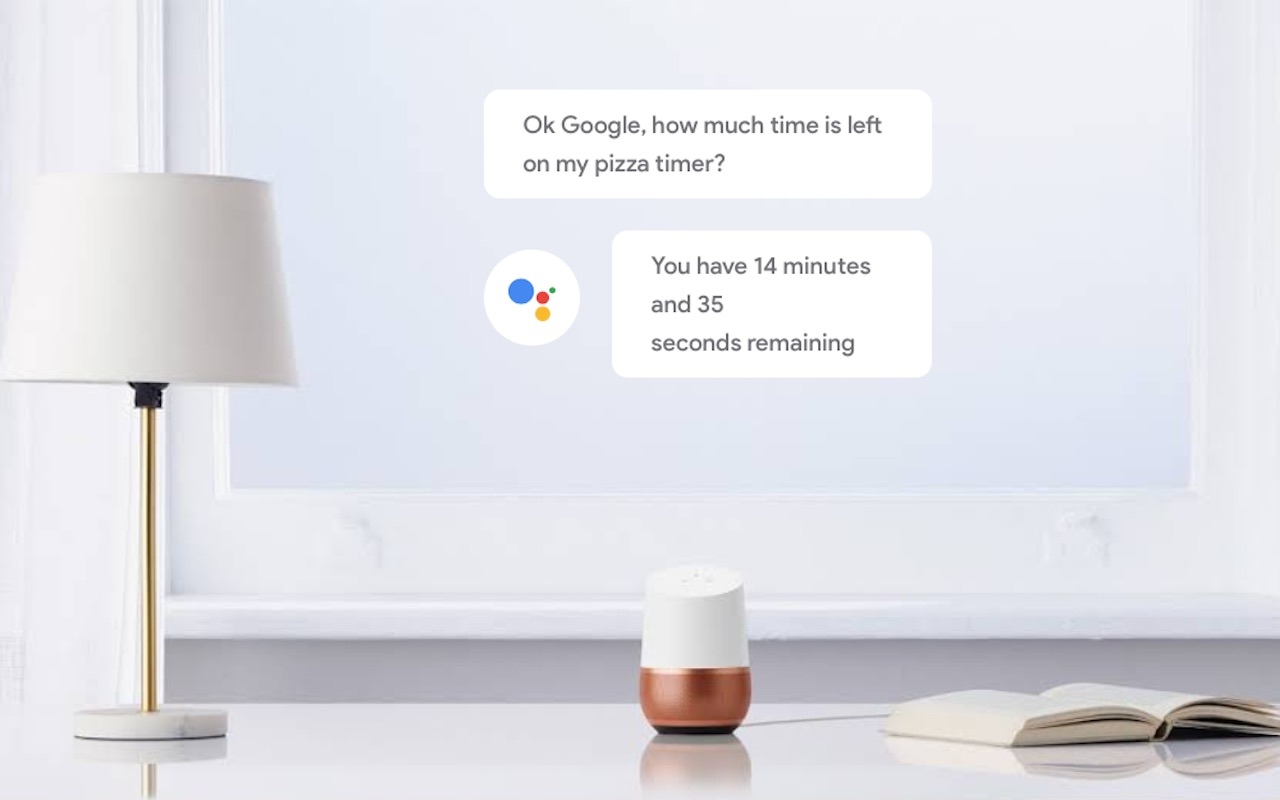
\includegraphics{figure/speech_goog.jpg}}
\end{figure}
\textbf{Speech Recognition and Generation} (e.g. google assistant)
Neural network extracts features from audio data in order to classify emotions in speech.
\end{frame}
%%%%%%%%%%%%%%%%%%%%%%%%%%%%%%%%%%%%%%%%%%%%%%%%%%%%%%%%%%%%%%%%%%

\endlecture
\end{document}